\subsection{Mokymosi greičio įtaka rezultatams}
\label{subsec:mokymosi_greicio_itaka}

Buvo ištirtos keturios mokymosi greičio reikšmės: $0{,}01$, $0{,}1$, $0{,}5$ ir $0{,}9$. Rezultatai pateikti~\ref{tab:lr_comparison} lentelėje.

\begin{table}[H]
    \centering
    \caption{Mokymosi greičio įtaka validavimo tikslumui ($500$ epochų).}
    \begin{tabular}{|c|c|c|}
        \hline
        $\eta$ & BGN validavimo tikslumas & SGN validavimo tikslumas \\
        \hline
        $0{,}01$ & $81{,}8\ \%$ & $99{,}1\ \%$ \\ \hline
        $0{,}1$ & $98{,}2\%$ & $99{,}1\ \%$ \\ \hline
        $0{,}5$ & $98{,}2\ \%$ & $99{,}1\ \%$ \\ \hline
        $0{,}9$ & $98{,}2\ \%$ & $99{,}1\ \%$ \\ \hline
    \end{tabular}
    \label{tab:lr_comparison}
\end{table}

Paketinis gradientinis nusileidimas yra jautresnis mokymosi greičio parinkimui – su $\eta = 0{,}01$ validavimo tikslumas siekia tik $81{,}8\ \%$, nes per $500$ epochų modelis nespėja pakankamai konverguoti. Didinant $\eta$ iki $0{,}1$ ir daugiau, tikslumas stabilizuojasi ties $98{,}2\ \%$ (žr.~\ref{fig:lr_comparison_bgd} pav.).

Stochastinis gradientinis nusileidimas yra atsparesnis mokymosi greičio pasirinkimui – visais keturiais atvejais pasiekiamas $99{,}1\ \%$ validavimo tikslumas (žr.~\ref{fig:lr_comparison_sgd} pav.).

\begin{figure}[H]
    \centering
    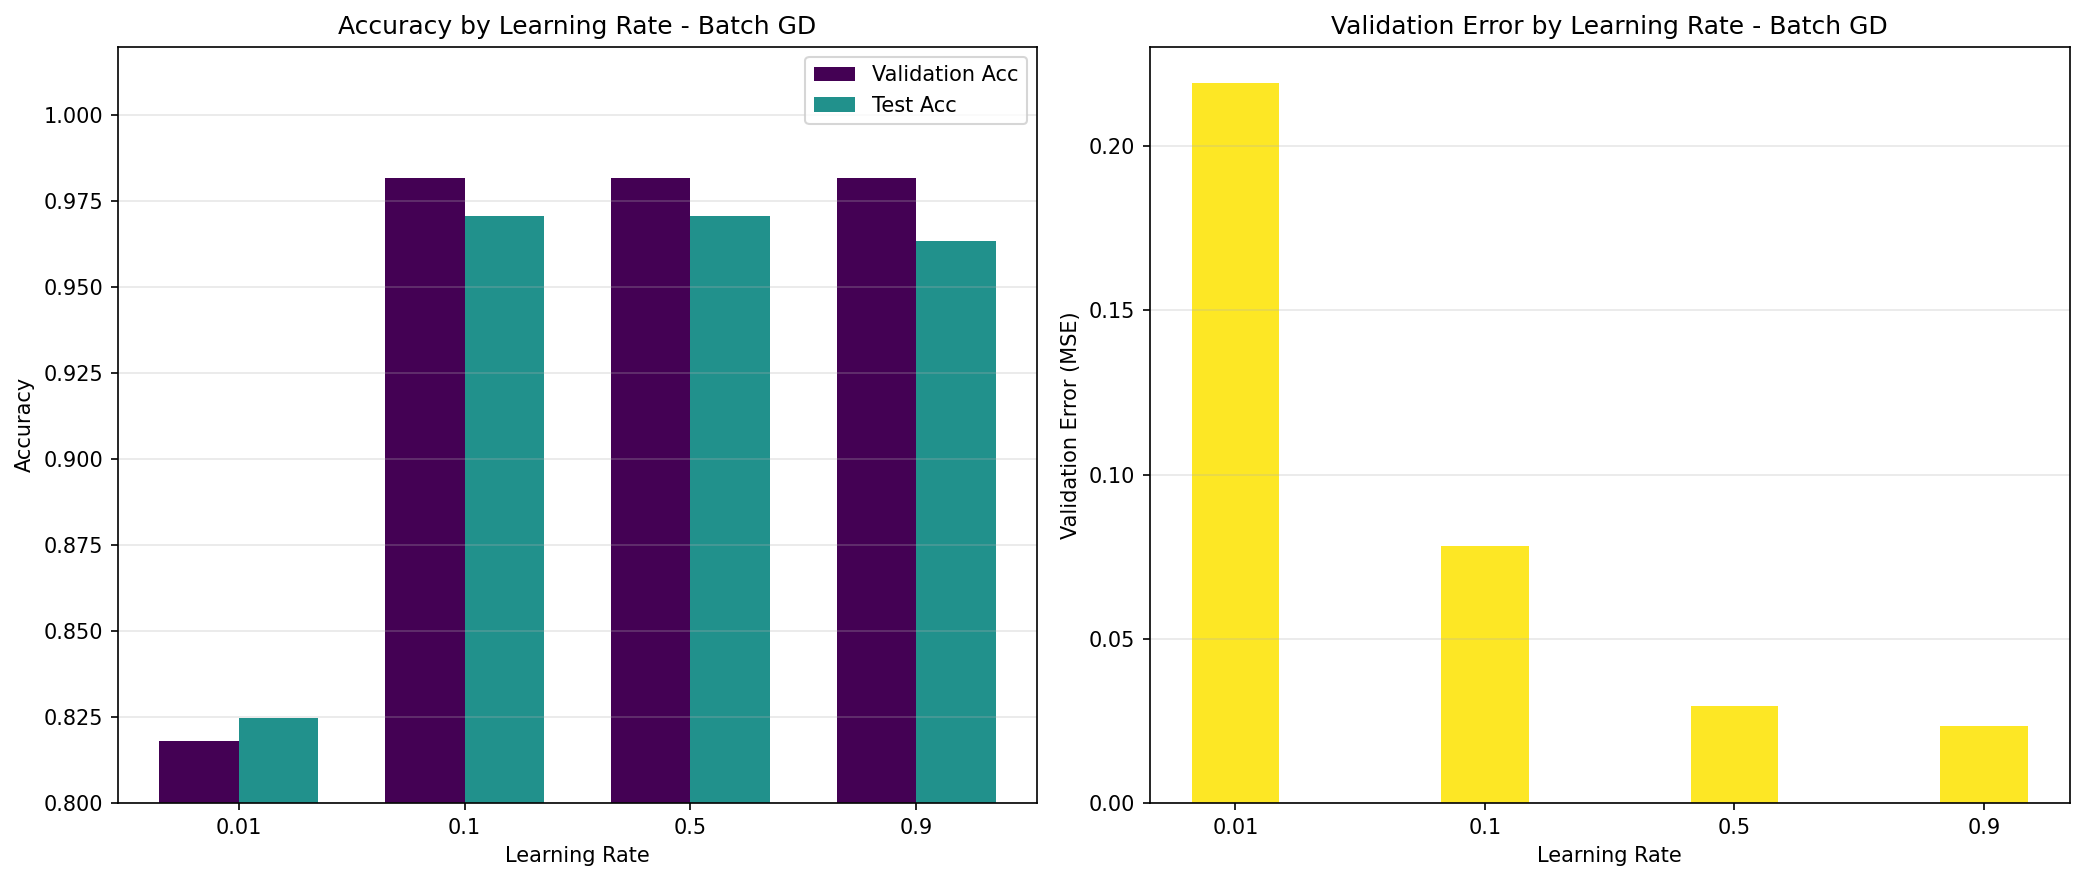
\includegraphics[width=0.85\linewidth]{2Lab/visualizations/lr_comparison_bgd.png}
    \caption{Mokymosi greičio įtaka rezultatams (paketinis GN)}
    \label{fig:lr_comparison_bgd}
\end{figure}

\begin{figure}[H]
    \centering
    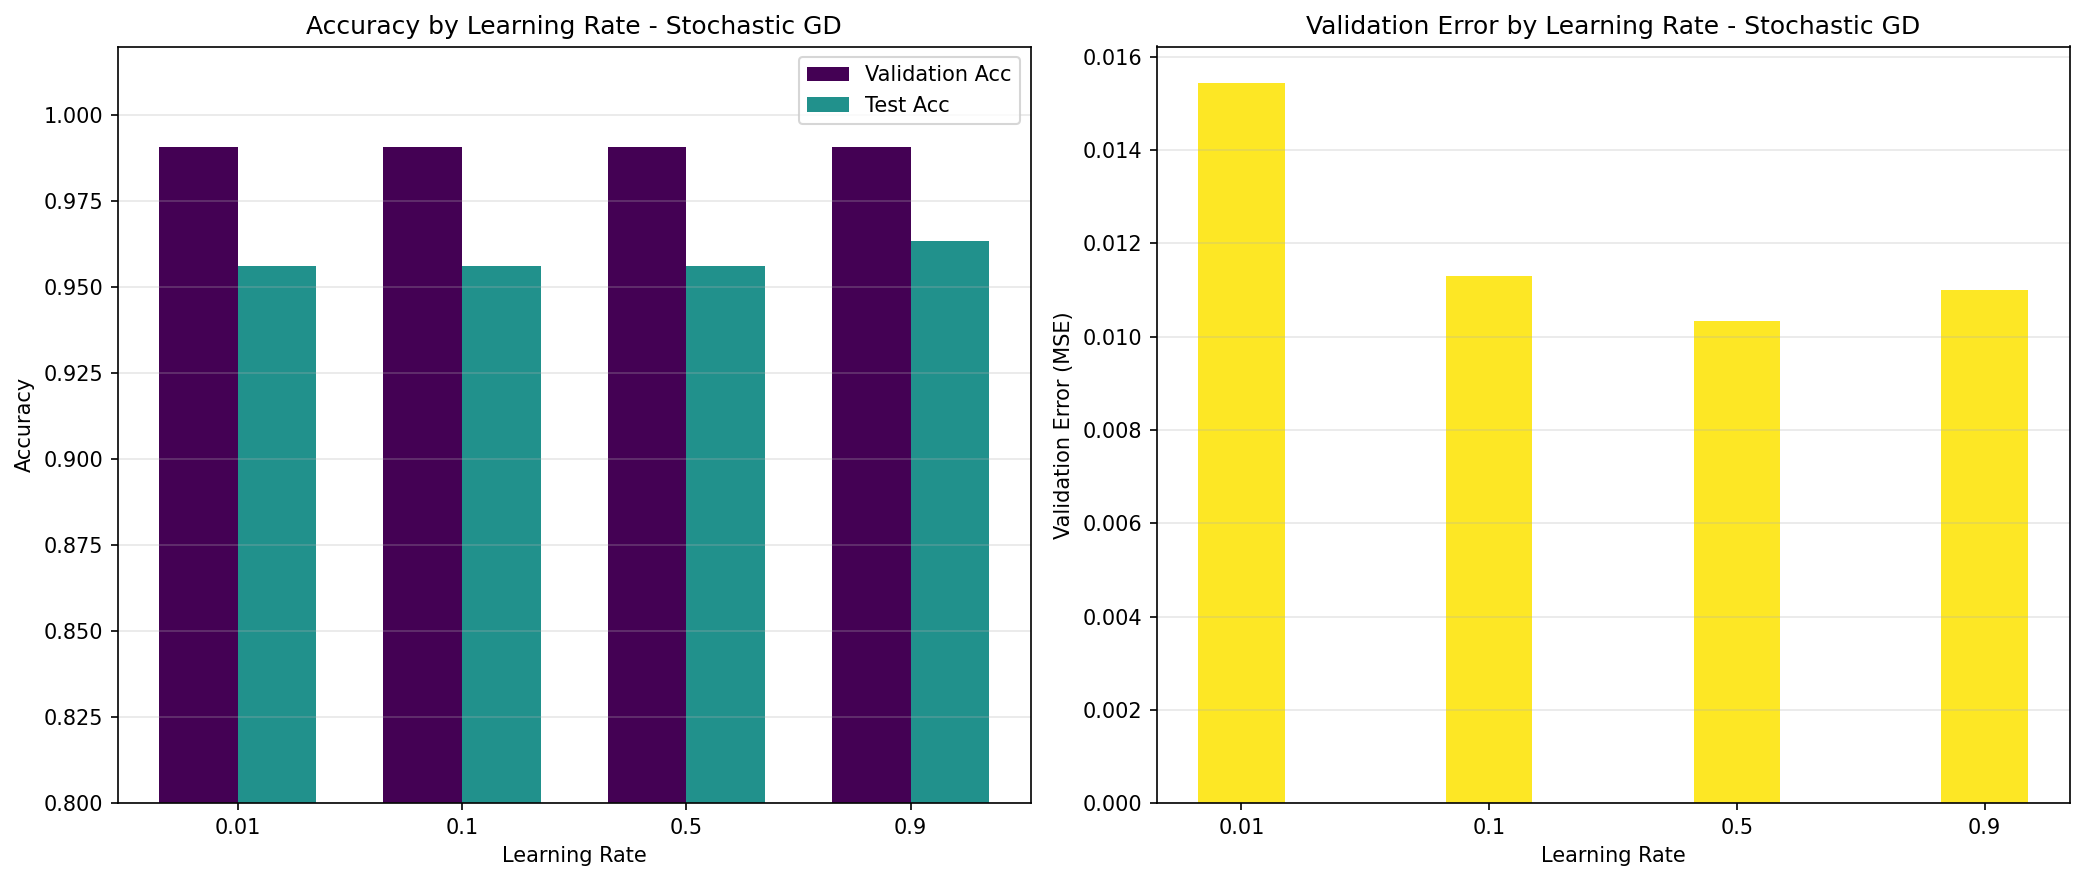
\includegraphics[width=0.85\linewidth]{2Lab/visualizations/lr_comparison_sgd.png}
    \caption{Mokymosi greičio įtaka rezultatams (stochastinis GN)}
    \label{fig:lr_comparison_sgd}
\end{figure}